\documentclass{article}
%\usepackage[spanish,activeacute]{babel}
%\usepackage[english,activeacute]{babel}
%\usepackage[latin1]{inputenc}
\usepackage[utf8]{inputenc}
\usepackage[english]{babel}

\usepackage{amsmath,amsfonts,amssymb,amstext,amsthm,amscd}
\usepackage{hyperref}
\usepackage{latexsym}
\usepackage{graphicx}
%\usepackage{subfigure}
\usepackage{subfig}
%\linespread{1.6}
\usepackage{float}
\usepackage{dcolumn}% Align table columns on decimal point(esto lo saque del ejemplo de revtex4)
\usepackage{bm}% bold math(esto lo saque del ejemplo de revtex4)
\newcounter{itemR}
\usepackage{here} %recordar usar el comando[H] para las gráficas que es el comando here en lugar de [h!]
\usepackage{fancyhdr}
%\usepackage{sidecap}
%\usepackage[spanish,activeacute]{babel}
\usepackage{multirow}
\usepackage{multicol}
\usepackage{array}
\usepackage{enumitem}
%\usepackage{booktabs}% para hacer tablas profesionales con \toprule

% ------------------------------------------------------------------------------------------------------------------------------------------------------

\usepackage{fancyhdr}
\setlength{\headheight}{15.2pt}
\usepackage[paperwidth=8.5in, paperheight=11.0in, top=1.0in, bottom=1.0in, left=1.0in, right=1.0in]{geometry}

\pagestyle{fancyplain}
\fancyhead[LE,RO]{Práctica $\#$12}
\fancyhead[CE,CO]{}
\fancyhead[RE,LO]{P23-FIS1012-12}
\fancyfoot[LE,RO]{\thepage}
\fancyfoot[CE,CO]{Laboratorio de Física, UDLAP}
\fancyfoot[RE,LO]{}

% ------------------------------------------------------------------------------------------------------------------------------------------------------
% ------------------------------------------------------------------------------------------------------------------------------------------------------
% ------------------------------------------------------------------------------------------------------------------------------------------------------

\begin{document}

\fancypagestyle{plain}{
   	\renewcommand{\headrulewidth}{1pt}
   	\renewcommand{\footrulewidth}{1pt}
}

\renewcommand{\footrulewidth}{1pt}
\renewcommand{\tablename}{Tabla}
\renewcommand{\figurename}{Figura}

% ------------------------------------------------------------------------------------------------------------------------------------------------------
% ------------------------------------------------------------------------------------------------------------------------------------------------------
% ------------------------------------------------------------------------------------------------------------------------------------------------------

\title{Ley de Faraday}
\author{\small{Luis Alberto Gil Bocanegra ID: 177410, Erick Gonzalez Parada ID: 178145}\\
 \small{Gartzen Aldecoa Barroso ID: 178034 .}\\		% ----- Varios autores separarlos por comas:  \small{Nombre(s) de (los) autor(es)\footnote{ID; correo@udlap.mx}, Nombre(s) de (los) autor(es)\footnote{ID; correo@udlap.mx}
	   \small{Depto. de Actuaría, Física y Matemáticas, Universidad de las Américas Puebla, Puebla, M\'exico 72810}}
\date{\small{\today}}

\maketitle

% ------------------------------------------------------------------------------------------------------------------------------------------------------
% ------------------------------------------------------------------------------------------------------------------------------------------------------
% ------------------------------------------------------------------------------------------------------------------------------------------------------

\begin{abstract}
Se observo el comportamiento de un imán rebotante
con esta oscilación del imán dentro de la bobina se midió el voltaje 
y se graficaron voltaje vs tiempo cuando solo un polo oscila y cuando ambos,
por ultimo se identificaron los máximos locales para graficarlos separadamente
resultando en gráficas con comportamientos correctos.
\\
\\
{\it Keywords:} Lineas de campo , corriente  
\\
\\
\end{abstract}

% ------------------------------------------------------------------------------------------------------------------------------------------------------

\begin{multicols}{2}
\section{Desarrollo teórico}\label{Desarrollo Teorico}                              	% -------------------- Introducción
Nuestro objetivo fue observar la interacción entre la corriente
, el angulo con respecto a un campo magnético que "rebota"
y encontrar la fuerza electromotriz con respecto a 
las leyes de Lens
\cite{Leskow}


La Ley de Inducción de Faraday describe cómo una variación en un campo magnético puede inducir una fuerza electromotriz (f.e.m.) en un circuito eléctrico circundante. Fue descubierta experimentalmente por el físico inglés Michael Faraday en 1831.


Según Faraday, la f.e.m. inducida en un circuito cerrado es directamente proporcional al ritmo de cambio del flujo magnético a través de la superficie delimitada por el circuito. Matemáticamente se expresa como:

\begin{equation}
\epsilon = - \frac{d\Phi_B}{dt}
\end{equation}

Donde $\epsilon$ es la f.e.m. inducida (en voltios), $\Phi_B$ es el flujo magnético (en webers) y $\frac{d\Phi_B}{dt}$ es la variación del flujo magnético con el tiempo (en webers/segundo). La constante de proporcionalidad se toma igual a -1 para cumplir la convención de signos en electromagnetismo.

La variación del flujo magnético con el tiempo induce corrientes eléctricas en el circuito que a su vez generan un campo magnético opuesto al cambio que las provocó. Esto se debe a que toda variación de un campo magnético induce una f.e.m. en cualquier circuito que lo intersecte. Las líneas de fuerza del campo cortan las de los electrones en movimiento y los empujan, generando la corriente eléctrica.



\section{Desarrollo Experimental}\label{Desarrollo experimental}				% -------------------- Metodología 
\subsection*{Lista de Materiales}
A continuación se presenta una lista de materiales:
\begin{enumerate}
    \item Fuente de bajo voltaje 0-24 V
    \item Nueces (3)
    \item Soporte universal (varilla y base)
    \item Imán cilíndrico 
    \item Resorte
    \item Bobina de Helmholtz 200 vueltas 
    \item Sensor de voltaje 
    \item Sensor de movimiento rotacional 
    \item Interfaz Universal 
    \item Varilla corta y vástagos(bobina y plástico) 
\end{enumerate}
Se procedió a montar el equipo de manera que el imán pueda oscilar dentro de la bobina. Posteriormente, se llevó a cabo la medición del voltaje inducido en la bobina durante este proceso.

Para visualizar los resultados de manera efectiva, se graficó el voltaje en función del tiempo en dos escenarios distintos:

En el primer escenario, se observa la oscilación cuando solo un polo del imán está en movimiento.
En el segundo escenario, se registra la oscilación cuando ambos polos del imán están en movimiento.

Posteriormente, se identificaron los máximos locales en ambas gráficas y se aplicó una línea de tendencia para una mejor interpretación de los datos. Este análisis proporcionará una comprensión más clara de la relación entre el movimiento del imán y el voltaje inducido en la bobina.
\end{multicols}
\section{Resultados y análisis}\label{Resultados}			% -------------------- Resultados

\begin{figure}[H]
   \centering
   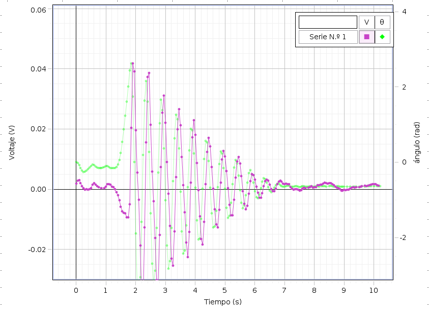
\includegraphics[scale=0.7]{../imgs/f.png}
   \caption{Un polo}
   \label{Fig:1}
\end{figure}

\begin{figure}[H]
   \centering
   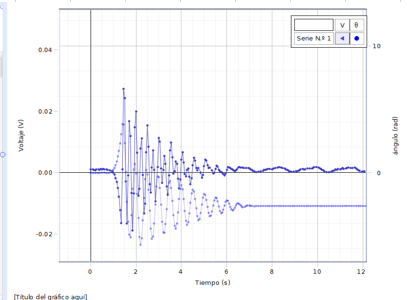
\includegraphics[scale=0.7]{../imgs/f0.png}
   \caption{Los dos polo}
   \label{Fig:2}
\end{figure}

La razón por la cual se presenta un zigzag en la gráfica de la figura \ref{Fig:2} en la que se miden los 2 polos del imán, es debido a que lo que busca el fenómeno con eso es mantener lo más estable posible la densidad del flujo magnético, ya que al medirse ambos polos del imán, la densidad se ve afectada por lo que el propio campo realiza estos ajustes en la densidad para mantenerla constante.

\begin{figure}[H]
   \centering
   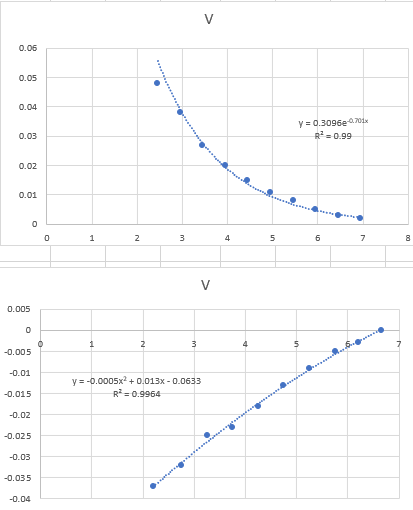
\includegraphics[scale=0.7]{../imgs/maxf.png}
   \caption{máximos de la \ref{Fig:1}}
   \label{Fig:3}
\end{figure}

\begin{figure}[H]
   \centering
   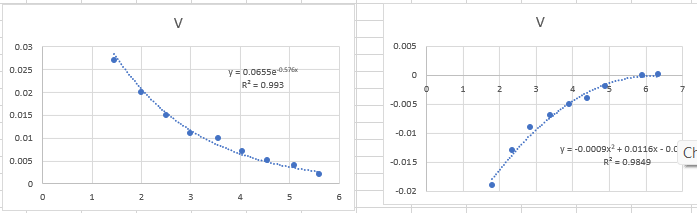
\includegraphics[scale=0.7]{../imgs/maxf0.png}
   \caption{máximos de la \ref{Fig:2}}
   \label{Fig:4}
\end{figure}


\section{Conclusiones}\label{Conclusiones}				% -------------------- Conclusiones
El objetivo si se cumplió, la teoría se asemejo muy bien a la práctica y como se pudo observar en las gráficas y como ya mencionado el comportamiento de nuestros datos es el correcto a excepción de cuando volteamos los polos, por otro lado y como ultimo comentario
La Ley de Inducción de Faraday establece que un cambio en el flujo magnético a través de un circuito induce una fuerza electromotriz (fem) en el mismo. Esta fem induce una corriente eléctrica cuando el circuito está cerrado. La magnitud de la fem inducida es proporcional a la rapidez con la que cambia el flujo magnético. En resumen, la ley de inducción de Faraday describe la relación entre la variación del campo magnético y la generación de corriente eléctrica, fundamental para entender los principios de los generadores eléctricos y otros dispositivos electromagnéticos. Esta ley es una piedra angular en la comprensión de la relación entre la electricidad y el magnetismo.

\begin{thebibliography}{9}						% -------------------- Bibliografía
	\bibitem{Leskow}
 Leskow, E. C. (2021, 15 julio). Ley de Faraday - concepto, historia, fórmula y ejemplos. Concepto. https://concepto.de/ley-de-faraday/
	\bibitem{Serway}
	Serway, R. A., $\&$ Jewett, J. W. (2008). Física para ciencias e ingeniería. (7.a
ed., Vol. 1). CENGAGE Learning.

\bibitem{Pérez}
	Newton, I. (1687). Philosophiæ Naturalis Principia Mathematica [Mathematical Principles of Natural Philosophy]. Londini: Jussu Societatis Regiæ ac Typis Josephi Streater.

\end{thebibliography}
\end{document}	